\section{Framework Design}

\begin{concept}{Framework Grundlagen}\\
Ein Framework ist ein Programmiergerüst mit folgenden Eigenschaften:
\begin{itemize}
    \item Bietet wiederverwendbare Funktionalität
    \item Definiert Erweiterungs- und Anpassungspunkte
    \item Verwendet Design Patterns
    \item Enthält keinen applikationsspezifischen Code
    \item Gibt Rahmen für anwendungsspezifischen Code vor
    \item Klassen arbeiten eng zusammen (vs. reine Bibliothek)
\end{itemize}
\end{concept}

\begin{definition}{Framework Entwicklung}\\
Die Entwicklung eines Frameworks erfordert:
\begin{itemize}
    \item Höhere Zuverlässigkeit als normale Software
    \item Tiefergehende Analyse der Erweiterungspunkte
    \item Hoher Architektur- und Designaufwand
    \item Sorgfältige Planung der Schnittstellen
\end{itemize}
\end{definition}

\begin{remark}{Kritische Betrachtung}\\
Herausforderungen beim Framework-Einsatz:
\begin{itemize}
    \item Frameworks tendieren zu wachsender Funktionalität
    \item Gefahr von inkonsistentem Design
    \item Funktionale Überschneidungen möglich
    \item Hoher Einarbeitungsaufwand
    \item Schwierige "Scheidung" nach Integration
    \item Trade-off zwischen Abhängigkeit und Nutzen
\end{itemize}
\end{remark}

\begin{KR}{Framework Design Principles}

\begin{minipage}[t]{0.5\textwidth}
\textbf{1. Abstraktionsebenen definieren}
\begin{itemize}
    \item \textbf{Core API:}
    \begin{itemize}
        \item Zentrale Interfaces
        \item Hauptfunktionalität
        \item Erweiterungspunkte
    \end{itemize}
    
    \item \textbf{Extensions:}
    \begin{itemize}
        \item Plugin-Mechanismen
        \item Callback-Interfaces
        \item Event-Systeme
    \end{itemize}
    
    \item \textbf{Implementierung:}
    \begin{itemize}
        \item Standard-Implementierungen
        \item Utility-Klassen
        \item Helper-Funktionen
    \end{itemize}
\end{itemize}
\end{minipage}
\begin{minipage}[t]{0.5\textwidth}
\textbf{2. Erweiterungsmechanismen}
\begin{itemize}
    \item \textbf{Interface-basiert:}
    \begin{itemize}
        \item Klare Verträge
        \item Lose Kopplung
        \item Einfache Erweiterung
    \end{itemize}
    
    \item \textbf{Annotations:}
    \begin{itemize}
        \item Deklarative Konfiguration
        \item Metadaten-getrieben
        \item Runtime-Processing
    \end{itemize}
    
    \item \textbf{Composition:}
    \begin{itemize}
        \item Plugin-System
        \item Service-Loader
        \item Dependency Injection
    \end{itemize}
\end{itemize}
\end{minipage}
\end{KR}

\begin{KR}{Analyse von Framework-Anforderungen}

\begin{minipage}[t]{0.5\textwidth}
\textbf{1. Fachliche Analyse}
\begin{itemize}
    \item \textbf{Core Features:}
    \begin{itemize}
        \item Zentrale Funktionalität
        \item Gemeinsame Abstraktionen
        \item Standardverhalten
    \end{itemize}
    \item \textbf{Variationspunkte:}
    \begin{itemize}
        \item Kundenspezifische\\ Anpassungen
        \item Optionale Features
        \item Erweiterungsmöglichkeiten
    \end{itemize}
\end{itemize}
\end{minipage}
\begin{minipage}[t]{0.5\textwidth}
\textbf{2. Technische Analyse}
\begin{itemize}
    \item \textbf{Architektur-Entscheidungen:}
    \begin{itemize}
        \item Erweiterungsmechanismen
        \item Integration in\\ bestehende Systeme
        \item Schnittstellen-Design
    \end{itemize}
    \item \textbf{Qualitätsanforderungen:}
    \begin{itemize}
        \item Performance
        \item Wartbarkeit
        \item Testbarkeit
    \end{itemize}
\end{itemize}
\end{minipage}
\end{KR}


\begin{example2}{Prüfungsaufgabe: Framework-Analyse}\\
\textbf{Szenario:}
Ein Framework für die Verarbeitung verschiedener Dokumentformate (PDF, DOC, TXT) 
soll entwickelt werden.

\textbf{Aufgabe:}
Analysieren Sie die Design-Entscheidungen.

\textbf{Lösung:}
\begin{itemize}
    \item \textbf{Erweiterungspunkte:}
    \begin{itemize}
        \item Dokumenttyp-Erkennung
        \item Parser für Formate
        \item Konvertierungslogik
    \end{itemize}
    
    \item \textbf{Design Patterns:}
    \begin{itemize}
        \item Factory für Parser-Erzeugung
        \item Strategy für Verarbeitungsalgorithmen
        \item Template Method für Konvertierung
    \end{itemize}
    
    \item \textbf{Schnittstellen:}
    \begin{itemize}
        \item DocumentParser Interface
        \item ConversionStrategy Interface
        \item DocumentMetadata Klasse
    \end{itemize}
\end{itemize}
\end{example2}



\subsection{Design Patterns in Frameworks}

\begin{concept}{Factory Method}\\
\textbf{Problem:} Flexible Objekterzeugung in wiederverwendbarer Klasse\\
\textbf{Lösung:}
\begin{itemize}
    \item Abstrakte Factory-Methode in Creator-Klasse
    \item Konkrete Subklassen überschreiben Methode
    \item Parallele Vererbungshierarchien
\end{itemize}
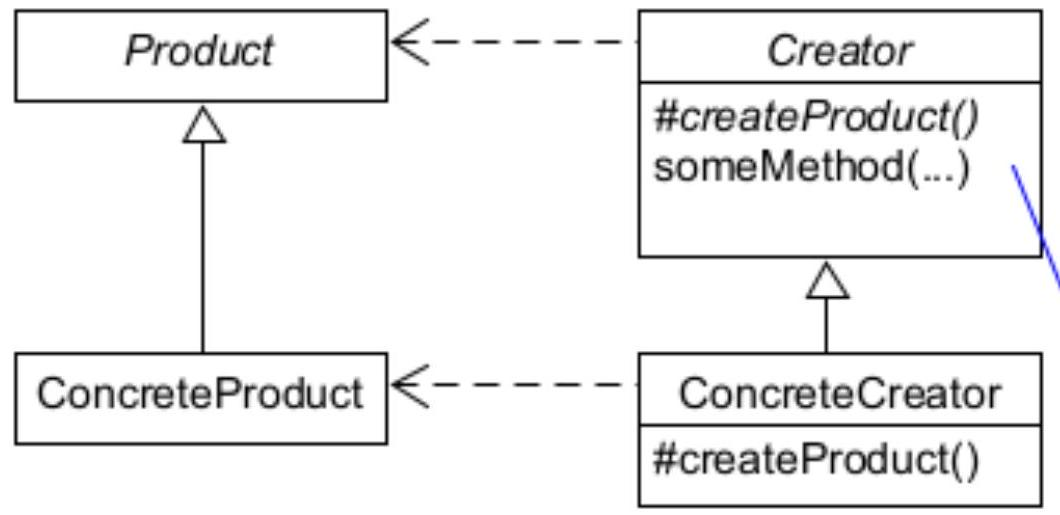
\includegraphics[width=0.6\linewidth]{images/2025_01_02_73d93f10fa91ab6123dcg-16}
\end{concept}

\begin{concept}{Abstract Factory}\\
\textbf{Problem:} Erzeugung verschiedener, zusammengehörender Objekte ohne Kenntnis konkreter Klassen\\
\textbf{Lösung:}
\begin{itemize}
    \item AbstractFactory-Interface definieren
    \item Pro Produkt eine create-Methode
    \item Konkrete Factories implementieren Interface
\end{itemize}
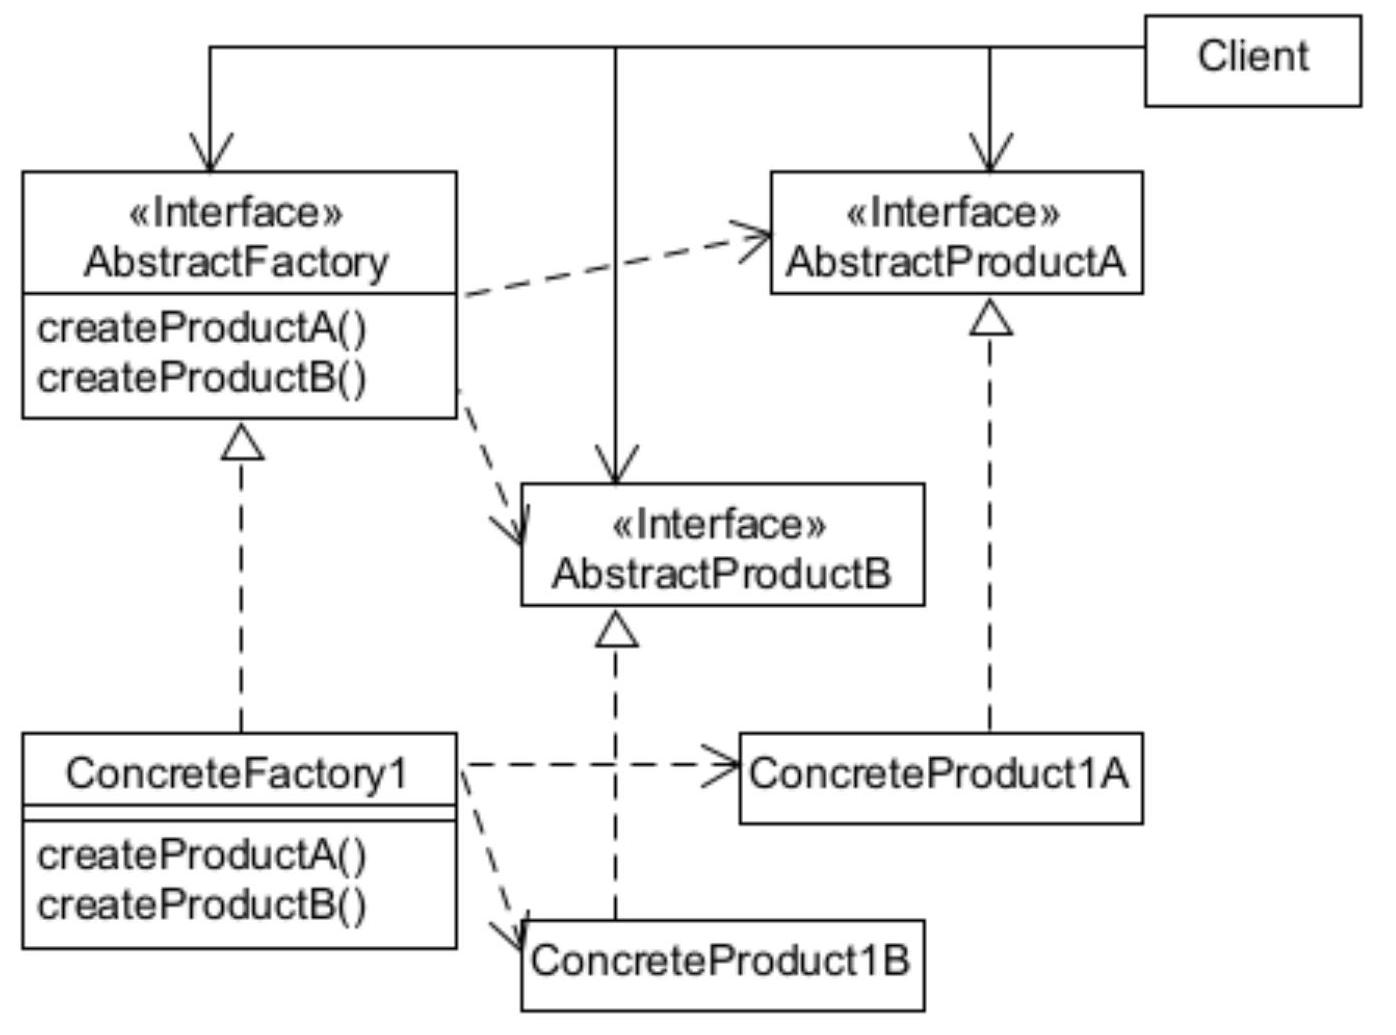
\includegraphics[width=0.8\linewidth]{images/2025_01_02_73d93f10fa91ab6123dcg-13}
\end{concept}


\begin{concept}{Command}\\
\textbf{Problem:} Aktionen für späteren Gebrauch speichern und verwalten\\
\textbf{Lösung:}
\begin{itemize}
    \item Command-Interface definieren
    \item Konkrete Commands implementieren
    \item Parameter für Ausführung speichern
    \item Optional: Undo-Funktionalität
\end{itemize}
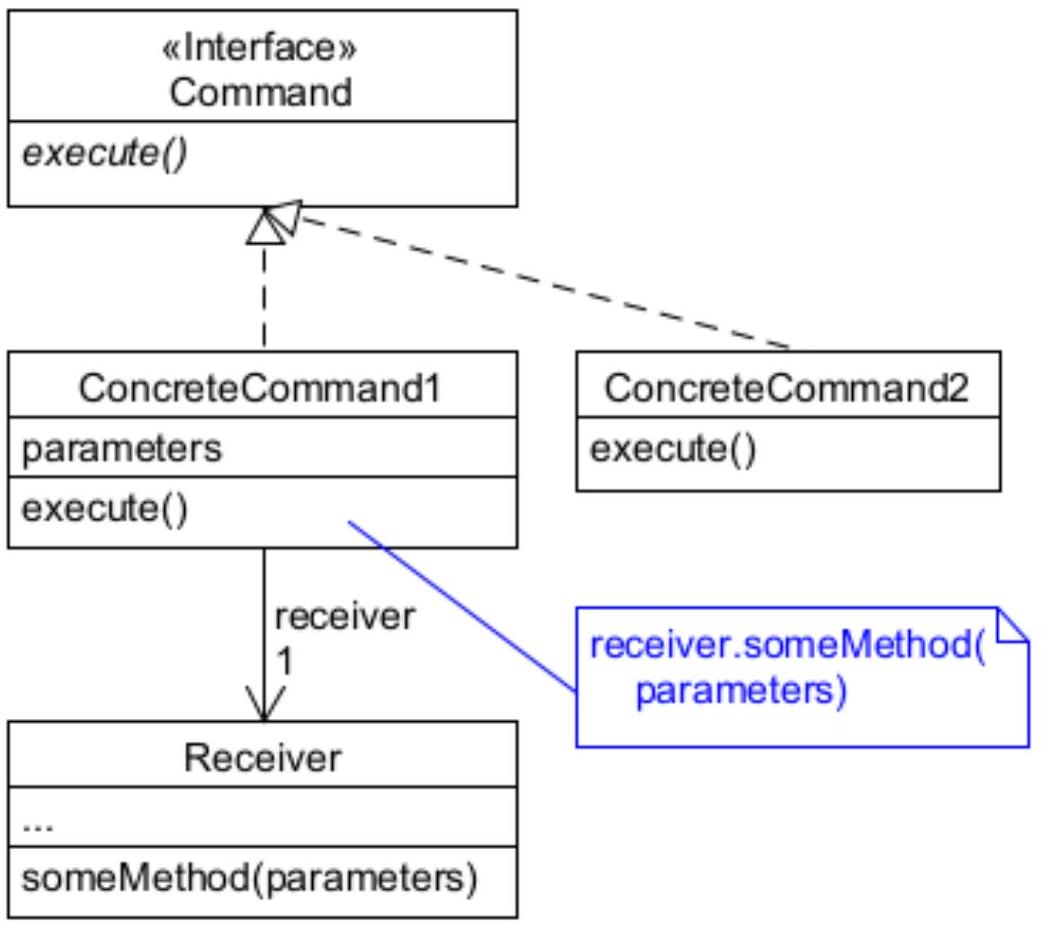
\includegraphics[width=0.7\linewidth]{images/2025_01_02_73d93f10fa91ab6123dcg-19}
\end{concept}


\begin{concept}{Template Method}\\
\textbf{Problem:} Algorithmus mit anpassbaren Teilschritten\\
\textbf{Lösung:}
\begin{itemize}
    \item Template Method in abstrakter Klasse
    \item Hook-Methoden für variable Teile
    \item Hollywood Principle: "Don't call us, we'll call you"
\end{itemize}
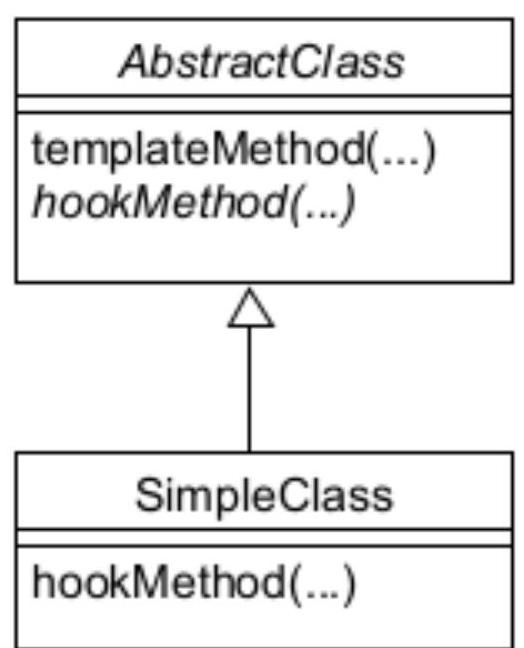
\includegraphics[width=0.3\linewidth]{images/2025_01_02_73d93f10fa91ab6123dcg-22}
\end{concept}

\begin{example2}{Framework Design Pattern Anwendung}\\
\textbf{Aufgabe:}
Implementieren Sie ein Plugin-System mit verschiedenen Design Patterns.

\textbf{Analyse der Pattern-Kombination:}
\begin{itemize}
    \item \textbf{Abstract Factory:}
    \begin{itemize}
        \item Plugin-Familie erzeugen
        \item Zusammengehörige Komponenten
        \item Austauschbare Implementierungen
    \end{itemize}
    
    \item \textbf{Template Method:}
    \begin{itemize}
        \item Plugin-Lifecycle definieren
        \item Standardablauf vorgeben
        \item Erweiterungspunkte bieten
    \end{itemize}
    
    \item \textbf{Command:}
    \begin{itemize}
        \item Plugin-Aktionen kapseln
        \item Asynchrone Ausführung
        \item Undo-Funktionalität
    \end{itemize}
\end{itemize}
\end{example2}


\subsection{Moderne Framework Mechanismen}

\begin{definition}{Annotation-basierte Konfiguration}\\
Moderne Frameworks nutzen Annotationen für:
\begin{itemize}
    \item Dependency Injection
    \item Konfiguration
    \item Interface-Implementation
    \item Funktionalitätserweiterung
\end{itemize}
\end{definition}

\begin{concept}{Annotations als Steuerungsmechanismus}\\
\textbf{Vorteile von Annotations:}
\begin{itemize}
    \item Keine harte Abhängigkeit zum Framework\\ (geringere Kopplung zur API)
    \item Annotation wird stillschweigend entfernt wenn nicht gefunden
    \item Geeignet für Domänenlogik ohne technische Abhängigkeiten
    \item Deklarativer Programmierstil
    \item Reduzierung von Boilerplate-Code
\end{itemize}

\textbf{Nachteil von Annotations:} Kann zu längeren Startzeiten führen
\end{concept}

\begin{theorem}{Auswertung von Annotations:}
\begin{itemize}
    \item \textbf{Startzeitpunkt:}
    \begin{itemize}
        \item Framework wird mit Anwendung gestartet
        \item Sucht Anwendungsklassen auf dem Klassenpfad
        \item Untersucht Annotationen
    \end{itemize}
    \item \textbf{Mögliche Framework-Aktionen:}
    \begin{itemize}
        \item Dependency Injection in Anwendungsobjekte
        \item Automatische Interface-Implementierung
        \item Funktionalität zu Klassen hinzufügen
    \end{itemize}
\end{itemize}
\end{theorem}

\begin{concept}{Aspekt-orientierte Programmierung in Frameworks}\\
\textbf{Querschnittliche Belange (Cross-Cutting Concerns):}
\begin{itemize}
    \item Logging
    \item Sicherheit
    \item Transaktionsmanagement
    \item Performance Monitoring
\end{itemize}

\textbf{Implementation mit Annotations:}
\begin{lstlisting}[language=Java, style=basesmol]
@Aspect
public class LoggingAspect {
    @Around("@annotation(Logged)")
    public Object logMethod(
            ProceedingJoinPoint joinPoint) 
            throws Throwable {
        
        String methodName = 
            joinPoint.getSignature().getName();
        Logger.info("Entering " + methodName);
        
        try {
            Object result = joinPoint.proceed();
            Logger.info("Exiting " + methodName);
            return result;
        } catch (Exception e) {
            Logger.error("Error in " + methodName, e);
            throw e;
        }
    }
}
// Usage in Framework Client Code
@Logged
public void businessMethod() {
    // Method implementation
}
\end{lstlisting}
\end{concept}



\begin{KR}{Java Mechanismen für Framework-Implementation}

    \begin{minipage}[t]{0.55\textwidth}
\textbf{1. Zeitpunkte für Code-Generierung}
\begin{itemize}
    \item \textbf{Compile-Zeit:}
    \begin{itemize}
        \item AnnotationProcessor
        \item Quellcode oder Bytecode generieren
    \end{itemize}
    \item \textbf{Laufzeit:}
    \begin{itemize}
        \item Beim Laden der Klassen
        \item Framework-Classloader
        \item Bytecode-Modifikation
    \end{itemize}
\end{itemize}
\end{minipage}
\begin{minipage}[t]{0.45\textwidth}
\textbf{2. Implementierungstechniken}
\begin{itemize}
    \item \textbf{Code Generation:}
    \begin{itemize}
        \item Quellcode hinzufügen
        \item Bytecode modifizieren
    \end{itemize}
    \item \textbf{Proxy Generation:}
    \begin{itemize}
        \item java.lang.reflect.Proxy
        \item Interface-Implementation
    \end{itemize}
\end{itemize}
\end{minipage}
\end{KR}

\begin{formula}{Framework Evaluation}

    \begin{minipage}[t]{0.5\textwidth}
\textbf{1. Qualitätskriterien}
\begin{itemize}
    \item \textbf{Usability:}
    \begin{itemize}
        \item Intuitive API
        \item Gute Dokumentation
        \item Beispiele/Templates
    \end{itemize}
    
    \item \textbf{Flexibilität:}
    \begin{itemize}
        \item Erweiterbarkeit
        \item Konfigurierbarkeit
        \item Modularität
    \end{itemize}
    
    \item \textbf{Wartbarkeit:}
    \begin{itemize}
        \item Klare Struktur
        \item Testbarkeit
        \item Versionierung
    \end{itemize}
\end{itemize}
\end{minipage}
\begin{minipage}[t]{0.5\textwidth}
\textbf{2. Risikobewertung}
\begin{itemize}
    \item \textbf{Technisch:}
    \begin{itemize}
        \item Kompatibilität
        \item Performance
        \item Skalierbarkeit
    \end{itemize}
    
    \item \textbf{Organisatorisch:}
    \begin{itemize}
        \item Learning Curve
        \item Support/Community
        \item Zukunftssicherheit
    \end{itemize}
\end{itemize}
\end{minipage}
\end{formula}

\begin{example2}{Prüfungsaufgabe: Framework Design Entscheidungen}\\
\textbf{Szenario:}
Sie sollen für eine Firma ein Framework zum Verarbeiten von Datenexporten entwickeln.
Die Firma arbeitet mit verschiedenen Datenformaten (CSV, Excel, XML) und möchte das 
Framework später einfach um weitere Formate erweitern können.

\textbf{Aufgabenstellung:}
\begin{enumerate}
    \item Identifizieren Sie die Variationspunkte
    \item Wählen Sie geeignete Design Patterns
    \item Skizzieren Sie die Framework-Architektur
\end{enumerate}

\textbf{Musterlösung:}
\begin{itemize}
    \item \textbf{Variationspunkte:}
    \begin{itemize}
        \item Format-Erkennung
        \item Datei-Parser
        \item Daten-Transformation
        \item Export-Ziele
    \end{itemize}
    
    \item \textbf{Design Patterns:}
    \begin{itemize}
        \item Abstract Factory für Parser-Erzeugung
        \item Strategy für unterschiedliche Parse-Algorithmen
        \item Template Method für generellen Export-Workflow
        \item Chain of Responsibility für Format-Erkennung
    \end{itemize}
    
    \item \textbf{Framework-Architektur:}
    \begin{itemize}
        \item Core API mit Interfaces
        \item Plugin-System für neue Formate
        \item Event-System für Export-Status
        \item Konfigurationsschicht
    \end{itemize}
\end{itemize}
\end{example2}

\columnbreak

\begin{example2}{Framework Design Pattern Kombination}\\
\textbf{Aufgabe:} 
Analysieren Sie die Kombination verschiedener Design Patterns in einem Framework.

\textbf{Muster-Framework:}
Event-Processing Framework mit folgenden Patterns:

\textbf{1. Template Method}
\begin{itemize}
    \item Definiert Workflow für Event-Verarbeitung
    \item Hook-Methoden für:
    \begin{itemize}
        \item Event-Validierung
        \item Event-Transformation
        \item Event-Persistierung
    \end{itemize}
\end{itemize}

\textbf{2. Chain of Responsibility}
\begin{itemize}
    \item Event-Handler-Kette
    \item Flexible Verarbeitungsreihenfolge
    \item Dynamische Handler-Registration
\end{itemize}

\textbf{3. Command}
\begin{itemize}
    \item Kapselung von Event-Handling-Logik
    \item Queuing von Events
    \item Undo/Redo Funktionalität
\end{itemize}

\textbf{4. Observer}
\begin{itemize}
    \item Benachrichtigung über Event-Status
    \item Lose Kopplung zwischen Komponenten
    \item Flexible Registration von Listeners
\end{itemize}

\textbf{Pattern-Interaktion:}
\begin{itemize}
    \item Template Method definiert Grundstruktur
    \item Chain of Responsibility organisiert Handler
    \item Command kapselt konkrete Aktionen
    \item Observer informiert über Ergebnisse
\end{itemize}
\end{example2}

\begin{example2}{Prüfungsaufgabe: Framework Testing}\\
\textbf{Szenario:}
Ein Framework soll gründlich getestet werden. Entwickeln Sie eine Teststrategie.

\textbf{Testebenen:}
\begin{itemize}
    \item \textbf{Unit Tests:}
    \begin{itemize}
        \item Einzelne Komponenten
        \item Mock-Objekte für Dependencies
        \item Edge Cases
    \end{itemize}
    
    \item \textbf{Integration Tests:}
    \begin{itemize}
        \item Zusammenspiel der Komponenten
        \item Plugin-Mechanismen
        \item Event-Handling
    \end{itemize}
    
    \item \textbf{System Tests:}
    \begin{itemize}
        \item End-to-End Szenarien
        \item Performance Tests 
        \item Load Tests
    \end{itemize}
\end{itemize}

\textbf{Besondere Aspekte:}
\begin{itemize}
    \item Extension Points testen
    \item Verschiedene Konfigurationen
    \item Backward Compatibility
    \item Error Handling
\end{itemize}
\end{example2}

\columnbreak

\begin{KR}{Framework-Extensions entwickeln}\\
\textbf{1. Extension Points identifizieren}
\begin{itemize}
    \item Core-Funktionalität analysieren
    \item Variationspunkte bestimmen
    \item Interface-Hierarchie planen
\end{itemize}

\textbf{2. Extension Mechanismen}
\begin{itemize}
    \item \textbf{Interface-basiert:}
    \begin{lstlisting}[language=Java, style=basesmol]
public interface Plugin {
    void initialize();
    void shutdown();
    String getName();
}
    \end{lstlisting}
    
    \item \textbf{Annotation-basiert:}
    \begin{lstlisting}[language=Java, style=basesmol]
@Extension
public class CustomPlugin {
    @Initialize
    public void setup() { ... }
    
    @Shutdown
    public void cleanup() { ... }
}
    \end{lstlisting}
\end{itemize}

\textbf{3. Discovery Mechanism}
\begin{lstlisting}[language=Java, style=basesmol]
public class ExtensionLoader {
    public List<Plugin> loadPlugins() {
        ServiceLoader<Plugin> loader = 
            ServiceLoader.load(Plugin.class);
        return StreamSupport
            .stream(loader.spliterator(), false)
            .collect(Collectors.toList());
    }
}
\end{lstlisting}
\end{KR}

\begin{example2}{Prüfungsaufgabe: Framework Evolution}\\
\textbf{Ausgangslage:}
Ein bestehendes Framework soll um neue Funktionalität erweitert werden, ohne bestehende 
Clients zu beeinträchtigen.

\textbf{Analyse der Optionen:}
\begin{itemize}
    \item \textbf{Annotation-basierte Erweiterung:}
    \begin{itemize}
        \item Vorteile:
        \begin{itemize}
            \item Keine Änderung bestehender Interfaces
            \item Optionale Funktionalität
            \item Deklarativer Ansatz
        \end{itemize}
        \item Nachteile:
        \begin{itemize}
            \item Komplexere Verarbeitung
            \item Mögliche Performance-Einbußen
            \item Schwieriger zu debuggen
        \end{itemize}
    \end{itemize}
    
    \item \textbf{Interface-basierte Erweiterung:}
    \begin{itemize}
        \item Vorteile:
        \begin{itemize}
            \item Klare Kontrakte
            \item Compile-time Checks
            \item Einfache Dokumentation
        \end{itemize}
        \item Nachteile:
        \begin{itemize}
            \item Änderungen an Interfaces nötig
            \item Adapter für alte Clients
            \item Höherer Implementierungsaufwand
        \end{itemize}
    \end{itemize}
\end{itemize}
\end{example2}

\columnbreak

\begin{KR}{Framework Integration}
\begin{enumerate}
    \item \textbf{Convention over Configuration}
    \begin{itemize}
        \item Namenskonventionen einhalten
        \item Standard-Verhalten nutzen
        \item Nur Ausnahmen konfigurieren
    \end{itemize}
    
    \item \textbf{Dependency Injection}
    \begin{itemize}
        \item Abhängigkeiten deklarieren
        \item Framework übernimmt Injection
        \item Constructor- oder Setter-Injection
    \end{itemize}
    
    \item \textbf{Interface-basierte Entwicklung}
    \begin{itemize}
        \item Interfaces definieren
        \item Framework generiert Implementation
        \item Methodennamen als Spezifikation
    \end{itemize}
\end{enumerate}
\end{KR}




\begin{example2}{Framework Integration Case Study}\\
\textbf{Szenario:}
Integration eines Logging-Frameworks in eine bestehende Anwendung

\textbf{Anforderungen:}
\begin{itemize}
    \item Minimale Änderungen am bestehenden Code
    \item Konfigurierbare Log-Level
    \item Verschiedene Log-Ausgaben (Konsole, File, DB)
    \item Performance-Monitoring
\end{itemize}

\textbf{Lösung mit Framework Patterns:}
\begin{lstlisting}[language=Java, style=basesmol]
// Logger Interface
public interface Logger {
    void debug(String message);
    void info(String message);
    void error(String message, Throwable t);
}
// Abstract Factory fuer Logger
public interface LoggerFactory {
    Logger getLogger(Class<?> clazz);
}
// Decorator fuer Performance Monitoring
public class PerformanceLogger implements Logger {
    private final Logger delegate;
    private final MetricsCollector metrics;
    
    @Override
    public void info(String message) {
        long start = System.nanoTime();
        try {
            delegate.info(message);
        } finally {
            long duration = System.nanoTime() - start;
            metrics.recordLogDuration(duration);
        }
    }
    // Other methods...
}
// Framework Configuration
@Configuration
public class LoggingConfig {
    @Bean
    public LoggerFactory loggerFactory(
            MetricsCollector metrics) {
        return clazz -> {
            Logger baseLogger = // create base logger
            return new PerformanceLogger(
                baseLogger, metrics);
        };
    }
}
\end{lstlisting}
\end{example2}

\columnbreak

\begin{example2}{Typische Prüfungsaufgabe: Framework Migration}\\
\textbf{Szenario:}
Ein bestehendes System soll von einem proprietären Framework auf ein Standard-Framework 
migriert werden.

\textbf{Aufgabenstellung:}
\begin{itemize}
    \item Analysieren Sie die Herausforderungen
    \item Entwickeln Sie eine Migrationsstrategie
    \item Bewerten Sie Risiken
\end{itemize}

\textbf{Lösungsansatz:}
\begin{itemize}
    \item \textbf{Analyse:}
    \begin{itemize}
        \item Framework-Abhängigkeiten identifizieren
        \item Geschäftskritische Funktionen isolieren
        \item Testabdeckung prüfen
    \end{itemize}
    
    \item \textbf{Strategie:}
    \begin{itemize}
        \item Adapter für Framework-Bridging
        \item Schrittweise Migration
        \item Parallelbetrieb ermöglichen
    \end{itemize}
    
    \item \textbf{Risikominimierung:}
    \begin{itemize}
        \item Automated Testing
        \item Feature Toggles
        \item Rollback-Möglichkeit
    \end{itemize}
\end{itemize}
\end{example2}









\subsubsection{complete examples}

\begin{example2}{Framework Design: Validation Framework}\\
\textbf{Anforderungen:}
Ein Framework für Validierung von Geschäftsobjekten soll entwickelt werden.

\textbf{Design:}
\begin{lstlisting}[language=Java, style=basesmol]
// Validation Annotations
@Target(ElementType.FIELD)
@Retention(RetentionPolicy.RUNTIME)
public @interface NotNull {
    String message() default "Value cannot be null";
}

@Target(ElementType.FIELD)
@Retention(RetentionPolicy.RUNTIME)
public @interface Length {
    int min() default 0;
    int max() default Integer.MAX_VALUE;
    String message() default "Length must be between {min} and {max}";
}

// Business Object
public class Customer {
    @NotNull
    private String id;
    
    @NotNull
    @Length(min = 2, max = 50)
    private String name;
    
    // getters and setters
}

// Validator Interface
public interface Validator<T> {
    ValidationResult validate(T object);
}

// Framework Implementation
public class ValidationFramework {
    public static <T> ValidationResult validate(T object) {
        Class<?> clazz = object.getClass();
        ValidationResult result = new ValidationResult();
        
        for (Field field : clazz.getDeclaredFields()) {
            validateField(object, field, result);
        }
        
        return result;
    }
}
\end{lstlisting}

\textbf{Verwendung:}
\begin{lstlisting}[language=Java, style=basesmol]
Customer customer = new Customer();
customer.setName("J"); // too short

ValidationResult result = 
    ValidationFramework.validate(customer);
if (!result.isValid()) {
    System.out.println(result.getErrors());
}
\end{lstlisting}
\end{example2}

\begin{example2}{Framework Design Pattern: Event System}\\
\textbf{Anforderung:}
Ein Framework soll Benutzern ermöglichen, auf verschiedene Events zu reagieren.

\textbf{Implementation:}
\begin{lstlisting}[language=Java, style=basesmol]
// Event Base Class
public abstract class Event {
    private final LocalDateTime timestamp;
    
    protected Event() {
        this.timestamp = LocalDateTime.now();
    }
    
    public LocalDateTime getTimestamp() {
        return timestamp;
    }
}

// Concrete Event
public class UserCreatedEvent extends Event {
    private final String userId;
    
    public UserCreatedEvent(String userId) {
        this.userId = userId;
    }
}

// Event Listener Interface
public interface EventListener<T extends Event> {
    void onEvent(T event);
}

// Event Bus
public class EventBus {
    private Map<Class<? extends Event>, 
               List<EventListener>> listeners = new HashMap<>();
    
    public <T extends Event> void register(
            Class<T> eventType, 
            EventListener<T> listener) {
        listeners.computeIfAbsent(eventType, 
            k -> new ArrayList<>()).add(listener);
    }
    
    public void publish(Event event) {
        List<EventListener> eventListeners = 
            listeners.get(event.getClass());
        if (eventListeners != null) {
            eventListeners.forEach(
                listener -> listener.onEvent(event));
        }
    }
}
\end{lstlisting}

\textbf{Framework Nutzung:}
\begin{lstlisting}[language=Java, style=basesmol]
// Framework Usage
EventBus eventBus = new EventBus();

// Register Listener
eventBus.register(UserCreatedEvent.class, 
    event -> System.out.println("User created: " 
        + event.getUserId()));

// Publish Event
eventBus.publish(new UserCreatedEvent("user123"));
\end{lstlisting}
\end{example2}